\section{Sprint 5}

\subsection*{Summary}

\begin{table}[H]
	\centering
	\begin{tabular}{ll}
		\toprule
		\multicolumn{2}{c}{\textbf{Sprint 5}}\\
		\midrule
		\textbf{Periode} & 13.04.2015 12:00 Uhr\textendash 27.04.2015 12:00 Uhr\\
		\textbf{Stunden Soll} & \SI{144}{\hour}\\
		\textbf{Stunden Plan} & \SI{154}{\hour} \\
		\textbf{Stunden Ist} & \SI{176.4}{\hour}\\
		\bottomrule
	\end{tabular}
\end{table}

\begin{figure}[H]
	\centering
	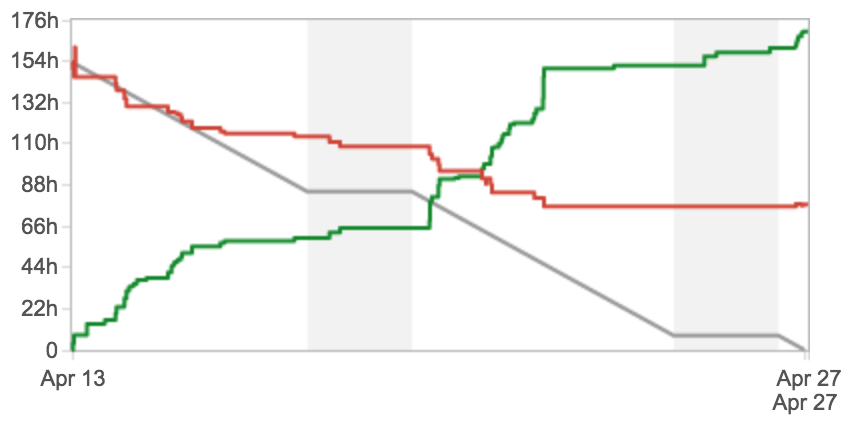
\includegraphics{fig/bd-sprint-5}
	\label{fig:pm:bd-sprint-5}
	\caption*{Burndown Chart Sprint 5}
\end{figure}

\subsection*{Ziele}
In diesem Sprint sollte einerseits die Performance durch Implementation von Caching Mechanismen gesteigert werden. Andererseits sollten Online Datenquellen automatisch in einem konfigurierbaren Intervall aktualisiert werden.

\subsection*{Abgeschlossen}
Folgende High-level (ohne Subtasks) Jira Tasks wurden während Sprint 5 abgeschlossen. 

\begin{table}[H]
\centering
\begin{tabular}{ll}
	\toprule
	\textbf{JIRA-Key} & \textbf{Summary}\\
	\midrule
DAT-88 & Online-Daten auto-refresh\\
DAT-94 & Interlis Kompatibilität\\
DAT-95 & CRUD Transformationen\\
DAT-96 & Caching\\
DAT-97 & Übrige Aufwände Sprint 5\\
DAT-98 & Organisation, Planung \& Kommunikation Sprint 5\\
DAT-99 & Projektmeetings Sprint 5\\
	\bottomrule
\end{tabular}	
\end{table}

Neu werden alle eingelesenen (geparsten) Dateien in verschiedenen Caches abgelegt, was die Interaktion im User Interface erheblich verschnellert. Zudem werden \acs{wfs}-Datenquellen automatisch erkannt und können ebenfalls verwendet werden. Das User Interface zur Erstellung der Transformationen ist nach wie vor in Entwicklung.

\subsection*{Probleme}
Meinungsverschiedenheiten in Team. Diese konnten durch Diskussion beigelegt werden.
